\documentclass[aspectratio=169,11pt]{beamer}
\usetheme[progressbar=frametitle,numbering=fraction,block=fill]{metropolis}
\usepackage{booktabs}
\usepackage{array}
\newcolumntype{L}[1]{>{\raggedright\arraybackslash}p{#1}}
\usepackage{amsmath,amssymb}
\usepackage{tikz}
\usetikzlibrary{arrows.meta,positioning,calc,shapes.geometric,decorations.pathreplacing}
\usepackage{pgfplots}
\pgfplotsset{compat=1.17}
\usepackage{tcolorbox}

% Palette: deep sea navy, teal, amber accent
\definecolor{sea}{HTML}{0B2545}
\definecolor{teal}{HTML}{13838F}
\definecolor{foam}{HTML}{E6F2F3}
\definecolor{amber}{HTML}{E09F3E}
\definecolor{mute}{HTML}{8A9BA8}
\setbeamercolor{normal text}{fg=sea!90!black,bg=white}
\setbeamercolor{alerted text}{fg=amber!85!black}
\setbeamercolor{frametitle}{bg=sea,fg=white}
\setbeamercolor{progress bar}{fg=teal,bg=foam}
\setbeamercolor{title separator}{fg=teal}
\setbeamercolor{background canvas}{bg=white}
\setbeamercolor{block title}{bg=foam,fg=sea}
\setbeamercolor{block body}{bg=foam!45}
\setbeamercolor{section in toc}{fg=sea}
\makeatletter\setlength{\metropolis@frametitle@padding}{1.6ex}\makeatother

\newcommand{\gapbox}[3]{%
  \begin{tcolorbox}[colback=foam!60,colframe=foam!60,arc=2mm,boxrule=0pt,left=2mm,right=2mm,top=0.6mm,bottom=0.6mm,before skip=0.8mm,after skip=0.8mm]
  {\bfseries\color{teal}#1}\hspace{1mm}{\small\bfseries #2}\\
  {\footnotesize #3}
  \end{tcolorbox}}
\newcommand{\stat}[2]{%
  \begin{minipage}[t]{\linewidth}\centering
  {\fontsize{22}{24}\selectfont\bfseries\color{teal}#1}\\[1mm]
  {\small #2}
  \end{minipage}}

% Evidence labels: what each statement rests on
\newcommand{\evtag}[2]{\tikz[baseline=(t.base)]\node[fill=#1,text=white,rounded corners=0.7mm,inner xsep=1mm,inner ysep=0.35mm,font=\tiny\bfseries](t){#2};}
\newcommand{\claim}{\evtag{sea!75}{CLAIM}}
\newcommand{\sugg}{\evtag{teal}{SUGGESTED}}
\newcommand{\open}{\evtag{amber}{OPEN}}
\newcommand{\src}{\evtag{mute}{SOURCE}}
\newcommand{\simres}{\evtag{teal!55!sea}{SIMULATED}}

% Symbols used throughout
\newcommand{\Nsym}{N_{\mathrm{sym}}}
\newcommand{\Kup}{K_{\mathrm{upd}}}
\newcommand{\dtol}{d_{\mathrm{tol}}}
\newcommand{\etol}{e_{\mathrm{tol}}}
\newcommand{\Pset}{\mathcal{P}}

\newcommand{\eps}{\epsilon}

\title{Sensor-Aided Doppler Estimation\\for Underwater Acoustic Links}
\subtitle{Who estimates which Doppler, from what, at what cost --- for group discussion}
\date{12 October 2026 (results updated 13 October)}
\institute{Target: IEEE JSAC special issue on Next-Generation Underwater Acoustic Communication Systems (deadline 31 March 2027)\\[1mm]
\claim\ to be shown \quad \simres\ simulation result \quad \sugg\ design proposal \quad \open\ needs material, a proof or an experiment \quad \src\ found by search, not yet checked in full}

\begin{document}

\maketitle

% ===========================================================
\section{Main idea}

\begin{frame}{The ground rule: estimation is the contribution}
\begin{columns}[T]
\begin{column}{0.55\textwidth}
\small
\textbf{Contribution:} the Doppler \alert{estimation} --- who estimates which part, from which information, how accurately, at what cost (pilots, bits, search).

\medskip
\textbf{Taken as a tool:} the \alert{compensation}. Once the estimate is right, resampling along the estimated trajectory works.

\medskip
{\footnotesize Supported by field data: on a surface buoy, a good frame-level estimate plus standard compensation leaves a residual of 0.2 subcarrier spacings (Lee et al.\ 2026). The open question is how to get the estimate right where that is not enough, and cheaply.}
\end{column}
\begin{column}{0.41\textwidth}
\begin{tcolorbox}[colback=sea,colframe=sea,arc=2mm,coltext=white,before skip=0pt]
\footnotesize\raggedright
\textbf{Doppler of a link}\\[1mm]
$\eps(t)=\dfrac{\big(v_A(t)-v_B(t+\tau)\big)\cdot u}{c}$\\[2mm]
transmitter share $+$ receiver share $+$ slow share $+$ path-specific share\\[1mm]
{\color{foam}changed on 12 Oct 2026; the compensation-focused deck is archived}
\end{tcolorbox}
\end{column}
\end{columns}
\end{frame}

\begin{frame}{Each part of the Doppler is known best in a different place}
\scriptsize\setlength{\tabcolsep}{4pt}\renewcommand{\arraystretch}{1.1}
\begin{tabular}{@{}L{0.30\textwidth}L{0.36\textwidth}L{0.28\textwidth}@{}}
\toprule
\textbf{Part} & \textbf{Known best by} & \textbf{Reaches the receiver as}\\
\midrule
transmitter's motion during emission & transmitter's IMU, live & \alert{side information in the same packet} (E1), or applied at the transmitter\\
receiver's motion during reception & receiver's IMU, live & direct input\\
slow part, sensor drift, direction errors & the received signal (preamble, postamble, pilots) & signal estimates\\
surface-scattered, path-specific & nobody & a floor\\
\bottomrule
\end{tabular}

\medskip
\small Today every UWA receiver estimates \emph{all} of it from the received signal alone. \textbf{Proposal:} estimate each part where it is known and \alert{fuse} them at the receiver (E2).
\end{frame}

\begin{frame}{Phase 0: the transmitter's motion must travel with the packet}
\begin{columns}[T]
\begin{column}{0.56\textwidth}
\scriptsize\setlength{\tabcolsep}{3pt}
\begin{tabular}{@{}L{0.42\textwidth}L{0.25\textwidth}L{0.25\textwidth}@{}}
\toprule
\textbf{Real buoy motion} & \textbf{2.3--2.4\,s ahead} & \textbf{share $<$10\,s waves}\\
\midrule
CDIP Waverider (0.9\,m), 3 Pacific sites & 0.77--1.08 & 45--95\%\\
OOI surface buoys (3.3\,m, 4\,t), Oregon, Irminger & 0.76--0.93 & 70--94\%\\
\bottomrule
\end{tabular}

\smallskip
{\scriptsize Normalised error of the best linear prediction of velocity (1 = no better than the mean). Every 0.8\,s, 0.8\,s ahead: 0.27--0.47.}

\medskip
\simres\ {\scriptsize Estimates one round trip old: $-12$ to $-5$\,dB SIR at every range (0.5--4\,km).}
\end{column}
\begin{column}{0.40\textwidth}
\footnotesize
\textbf{Consequences}
\begin{itemize}\setlength{\itemsep}{1pt}
\item feedback of Doppler across a round trip \alert{fails} (this killed our earlier forecast design)
\item the transmitter's own motion, measured \alert{while it sends}, is never stale if it travels \emph{in the same packet}
\item the receiver's own motion is measured live
\end{itemize}
\end{column}
\end{columns}
\end{frame}

\begin{frame}{The proposal: E1 side information, E2 fusion, E3 who estimates what \sugg}
\begin{columns}[T]
\begin{column}{0.54\textwidth}
\footnotesize
\begin{description}\setlength{\itemsep}{2pt}
\item[E1] The transmitter carries its measured motion over the packet in the packet: a few quantised samples or coefficients. How many bits, and how the receiver reads them before it knows the Doppler.
\item[E2] The receiver fuses E1, its own IMU and preamble / pilot estimates in one smoother over the packet. Sensors narrow the search and replace most pilots; the signal corrects sensor drift.
\item[E3] Which part from which source, given sensor quality, latency, packet length and pilot budget (our placement results, reread).
\end{description}
\end{column}
\begin{column}{0.42\textwidth}
\footnotesize
\textbf{Candidate claim} \sugg: the first sensor-aided Doppler estimation for UWA links --- transmitter motion as in-packet side information, fused with the receiver's IMU and signal estimates; sized in bits and pilots; closed forms from estimation error to interference; real buoy motion.

\medskip
\textbf{Sending vs applying:} the same transmitter estimate can be sent (E1) or applied (transmit-side pre-compensation); both are compared.
\end{column}
\end{columns}
\end{frame}

% ===========================================================
\section{Gaps with the literature}

\begin{frame}{Related work (1): Doppler estimated from the signal alone}
\scriptsize\setlength{\tabcolsep}{3pt}\renewcommand{\arraystretch}{0.95}
\begin{tabular}{@{}L{0.30\textwidth}L{0.36\textwidth}L{0.30\textwidth}@{}}
\toprule
\textbf{Work} & \textbf{Estimation} & \textbf{Limit for us}\\
\midrule
Sharif et al., JOE 2000 & Chirps at both ends of the packet & One scale per packet\\
Li et al., JOE 2008 & Preamble scale + residual CFO & Frame-level; pilots for the residual\\
Mason et al., 2008 & Multicarrier preamble: detection, sync, scale & Signal only\\
Cho--Kim, IET Commun.\ 2026 & Constant acceleration from the cyclic prefix & $\approx$1\,s frames\\
Sun 2022; Hu 2024 & Kalman Doppler tracking (DSSS, FH-FSK) & Signal only, no motion prior\\
\textbf{Lee et al.\ 2026} (preprint) & 10.5\,h surface-buoy trial: frame scale + per-symbol CFO & per-symbol tracking gains only $\times$1.15 in PER at $\approx$9\,dB\\
\bottomrule
\end{tabular}

\vspace{1mm}
\footnotesize All estimate everything from the received signal. Lee et al.\ show it is enough in a noise-limited link (QPSK, 0.9\,s frames, sea state 3, one moving end): our regime must be stated against it.
\end{frame}

\begin{frame}{Related work (2): sensors, side information, radio analogues}
\scriptsize\setlength{\tabcolsep}{3pt}\renewcommand{\arraystretch}{0.92}
\begin{tabular}{@{}L{0.33\textwidth}L{0.33\textwidth}L{0.30\textwidth}@{}}
\toprule
\textbf{Work} & \textbf{Mechanism} & \textbf{What it lacks}\\
\midrule
Aubry 2019; Garin 2021; Choi et al.\ RA-L 2022 & Modem Doppler into navigation filters & Runs the other way\\
DE-Sync 2018, APE-Sync 2019 & Far end's Doppler returned in the reply & Only to set clocks\\
Oiwa et al., IEICE Tech.\ Rep.\ 2020 & Accelerometer-aided compensation & One end; not peer reviewed\\
3GPP NTN; US 10,826,595 & GNSS velocity $\to$ Doppler pre-compensation & Radio; ephemeris/GNSS\\
Gan, US 10,015,762 (UAV) & IMU $\to$ Doppler predistortion & Radio; patents\\
AsyMov, arXiv 2412.10387 & Channel Doppler vs IMU (ISAC) & IMU helps only when paths are scarce\\
\bottomrule
\end{tabular}

\vspace{1mm}
\footnotesize Local library, web and OpenAlex checked (9--12 Oct 2026): \alert{no UWA receiver uses motion sensors to estimate Doppler, and no transmitter sends its motion}. Radio precedents are mostly patents.
\end{frame}

\begin{frame}{Candidate gaps}
\gapbox{G1}{No UWA receiver uses motion sensors as an input to Doppler estimation}{Sensor + Doppler work feeds navigation (Aubry, Garin, Choi); only Oiwa 2020 at one end. Radio: GNSS / IMU-aided pre-compensation (NTN, UAV patents).}
\gapbox{G2}{No transmitter sends its motion; side-information size not analysed}{DE-Sync / APE-Sync exchange Doppler for clocks only; headers carry addresses, SNR, MCS.}
\gapbox{G3}{Accuracy / overhead / search trade-off with a sensor prior not analysed}{Signal-only estimators (Li 2008, Mason 2008, Cho--Kim 2026, Kalman trackers); Lee 2026 maps the noise-limited regime only.}
\gapbox{G4}{(Extension) multi-user branches estimated one by one}{Tu et al.\ 2011, 2013; per-user sensor priors unused.}
\end{frame}

% ===========================================================
\section{Evidence so far (reused)}

\begin{frame}{Sensor information is worth 4--15\,dB at the same pilot budget \simres}
\begin{columns}[T]
\begin{column}{0.58\textwidth}
\scriptsize\setlength{\tabcolsep}{3pt}\renewcommand{\arraystretch}{1.0}
\begin{tabular}{@{}L{0.40\textwidth}L{0.17\textwidth}L{0.17\textwidth}L{0.17\textwidth}@{}}
\toprule
\textbf{SIR [dB], 1\,s packets} & \textbf{Seabed CDIP} & \textbf{Seabed OOI} & \textbf{Buoy--buoy}\\
\midrule
Signal only, one estimate per symbol & 35.3 & 26.2 & 23.0\\
IMUs + one estimate per symbol & 39.3 & 38.4 & 37.8\\
IMUs + quadratic over all symbols & \textbf{43.9} & \textbf{41.0} & \textbf{39.6}\\
IMUs + 2 estimates per packet (line) & 39.8 & 37.1 & 36.0\\
\bottomrule
\end{tabular}

\smallskip
{\scriptsize Real buoy motion, 30 packets per point; IMU drift 0.01\,m/s, 50\,ms latency. With 20$^\circ$ path-direction error and 4\,s packets, IMUs + per-symbol estimates keep 30--39\,dB; 2 estimates per packet fall to 3--16\,dB.}
\end{column}
\begin{column}{0.38\textwidth}
\footnotesize
\begin{itemize}\setlength{\itemsep}{2pt}
\item same number of signal estimates, \alert{+4 / +12 / +15\,dB} with the sensors
\item sensors cover the fast motion; the signal covers drift and what sensors miss
\item this is E2 in its simplest form (sensor share + signal share, no proper fusion yet)
\end{itemize}
\end{column}
\end{columns}
\end{frame}

\begin{frame}{What the sensors must achieve \simres}
\begin{columns}[T]
\begin{column}{0.56\textwidth}
\scriptsize\setlength{\tabcolsep}{3pt}\renewcommand{\arraystretch}{0.95}
\begin{tabular}{@{}L{0.30\textwidth}L{0.33\textwidth}L{0.30\textwidth}@{}}
\toprule
\textbf{Factor} & \textbf{Sensors + 2 signal estimates} & \textbf{Sensors only}\\
\midrule
IMU drift 0.005 $\to$ 0.1\,m/s & 38--41 $\to$ 28--32 & 29--39 $\to$ 11\\
Latency 0 / 50 / 100 / 200\,ms & 42 / 37 / 30 / 20 & 32 / 33 / 28 / 16\\
\quad 50\,ms, not bridged & 25 & 17\\
Lever arm 2\,m, corrected / not & 38 / 13 & 31 / 3\\
Direction error 0 / 5 / 20$^\circ$ & 37 / 30 / 18 & 30 / 13 / 0\\
\bottomrule
\end{tabular}

\smallskip
{\scriptsize SIR [dB]; buoy$\to$seabed, OOI buoy.}
\end{column}
\begin{column}{0.40\textwidth}
\footnotesize
\textbf{Requirements on the sensor estimate}
\begin{itemize}\setlength{\itemsep}{1pt}
\item drift: up to $\approx$10$\times$ worse is fine when the signal corrects it
\item latency $\lesssim$100\,ms (0.01 wave periods), bridged by the accelerometer
\item lever arm from the gyro: mandatory
\item path direction within $\approx$5$^\circ$
\end{itemize}
\end{column}
\end{columns}
\end{frame}

\begin{frame}{Estimation error $\to$ interference, in closed form \simres}
\begin{columns}[T]
\begin{column}{0.50\textwidth}
\footnotesize
Interference = phase variance of the residual within each FFT window:
\[
I = (2\pi f_c)^2\,\overline{\mathrm{var}_{\mathrm{win}}\!\Big(\textstyle\int r\,dt\Big)}
\]
for any linear estimator (weights from its estimates to the trajectory).
\begin{itemize}\setlength{\itemsep}{1pt}
\item a residual \alert{ramp} costs 5$\times$ less than an offset of equal variance
\item 85 simulated points: right winner at 81 (misses $\le$0.6\,dB); every strategy within $\pm$0.7\,dB (median)
\end{itemize}
\textbf{Role now:} the metric that turns any estimation error (sensor, side information, pilots) into SIR.
\end{column}
\begin{column}{0.46\textwidth}
\footnotesize
\textbf{Validated sources of error}
\begin{itemize}\setlength{\itemsep}{1pt}
\item sensor drift, latency, lever arm, direction (node stage as a filter on the measured motion)
\item the fit the receiver really makes from its estimates
\item estimate noise through the fit's weights
\end{itemize}
Side-information quantisation (E1) and the fused covariance (E2) plug into the same formula.
\end{column}
\end{columns}
\end{frame}

\begin{frame}{A floor no estimate removes: surface-scattered Doppler \simres}
\centering
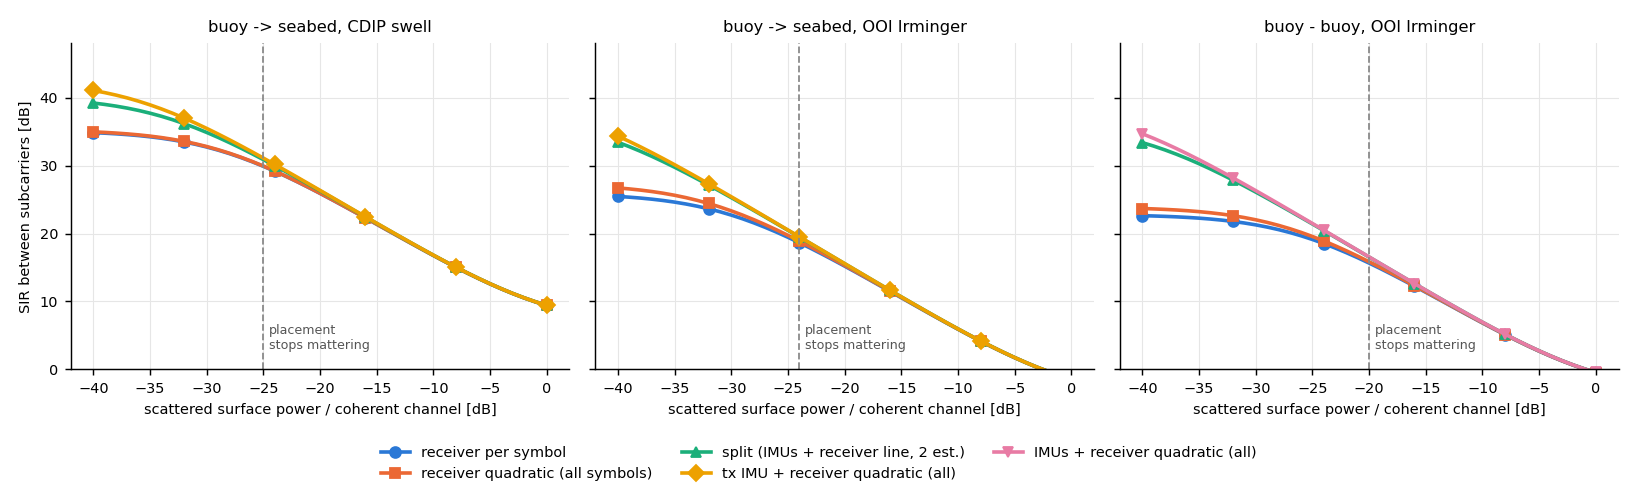
\includegraphics[width=0.97\textwidth]{../code/results/surface_scatter/sweep.png}

\footnotesize Better estimation pays only while the scattered surface power stays $\lesssim -20$ to $-25$\,dB below the coherent channel (Bellhop with measured roughness, scattered power swept). \open\ literature value for real channels.
\end{frame}

% ===========================================================
\section{Proposed methodology}

\begin{frame}{E1: Doppler side information \sugg\ (built)}
\begin{columns}[T]
\begin{column}{0.52\textwidth}
\footnotesize
\textbf{What:} the transmitter's velocity along the path over the packet, from its IMU (lever arm, latency handled at the source), as $K$ samples or polynomial / DCT coefficients, quantised to $B$ bits.

\medskip
\textbf{Where:} a robust low-rate header read after a coarse synchronisation (chicken and egg: the Doppler must be roughly known to read it), or carried by the preamble itself.

\medskip
\textbf{Output:} residual Doppler and SIR vs $B$; header failure vs SNR; compared with applying the estimate at the transmitter (no bits, one intended receiver) and with the receiver alone.
\end{column}
\begin{column}{0.44\textwidth}
\footnotesize
\textbf{Theory (T2):} residual variance vs bits from the motion spectrum: representation error (polynomial / sampled kernels, done) + quantisation noise $\to$ interference (T1).

\medskip
\textbf{Expected size:} a few coefficients per second of packet for wave motion (most energy below 0.3\,Hz) --- tens of bits, to be computed.

\medskip
\open\ header design; IMU access at symbol rate on real modems.
\end{column}
\end{columns}
\end{frame}

\begin{frame}{E2: fusion at the receiver \sugg\ (built)}
\begin{columns}[T]
\begin{column}{0.52\textwidth}
\footnotesize
\textbf{Smoother over the packet} (Kalman + RTS) on a wave-motion state: Doppler shares, rate, slow drift, IMU bias.

\textbf{Inputs:} E1 (with its quantisation error); own IMU samples (with latency); preamble / postamble / pilot measurements (SNR-dependent error).

\textbf{Output:} Doppler trajectory + covariance $\to$ resampler.

\medskip
\textbf{Gains to show:} accuracy at high SNR and long frames; pilots and preamble saved for a target SIR; narrower Doppler search (acquisition at low SNR); robustness when the signal estimate fails.
\end{column}
\begin{column}{0.44\textwidth}
\footnotesize
\textbf{Baselines}
\begin{itemize}\setlength{\itemsep}{0pt}
\item Li et al.\ 2008 two-step (preamble scale + residual CFO), as in Lee et al.\ 2026
\item per-symbol pilot tracking; signal-only Kalman
\item Cho--Kim constant acceleration
\end{itemize}
\textbf{Theory (T3):} Bayesian Cram\'er--Rao bound with and without the sensor prior, vs SNR and pilots.
\end{column}
\end{columns}
\end{frame}

% ===========================================================
\section{Results: the end-to-end chain}

\begin{frame}{What we built and compared \simres}
\begin{columns}[T]
\begin{column}{0.52\textwidth}
\footnotesize
\textbf{Frame:} up/down chirp \,|\, header (side information + CRC) \,|\, OFDM data (pilots, in-band nulls) \,|\, chirp. Rate-1/2 code, QPSK / 16-QAM, real pilot channel estimate, LLRs weighted by noise + interference on the nulls.

\medskip
\textbf{Channel:} real buoy motion (CDIP swell, OOI Irminger), unknown start, noise; Bellhop multipath with \alert{each path's own Doppler} from its angles.

\medskip
\textbf{Ours:} side information (16--96 bits) + own IMU $\to$ prior; Kalman fusion with postamble timing and per-symbol offsets; per-path cancellation with sensor-predicted Doppler.
\end{column}
\begin{column}{0.44\textwidth}
\footnotesize
\textbf{Baselines (state of the art)}
\begin{itemize}\setlength{\itemsep}{1pt}
\item Li et al.\ 2008 front end (as in Lee et al.\ 2026): preamble/postamble scale + per-symbol CFO
\item Cho--Kim 2026: constant acceleration from the cyclic prefix
\item \alert{signal-only Kalman}: our smoother without sensors (the strongest signal-only receiver)
\item Tu et al.-like multi-branch; signal-only cancellation (multipath)
\end{itemize}
{\scriptsize Two fixes made the comparison fair: chirp range--Doppler bias (up/down sweeps), and a wider CFO search for the baseline.}
\end{column}
\end{columns}
\end{frame}

\begin{frame}{Single path: where the sensors matter \simres}
\centering
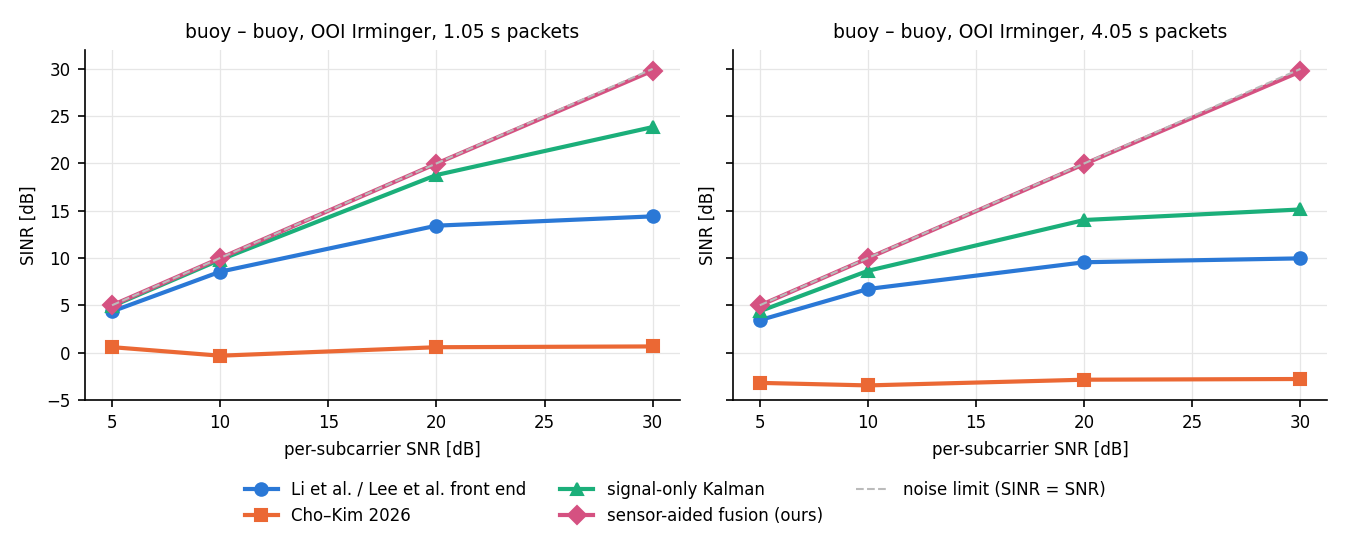
\includegraphics[width=0.88\textwidth]{../code/results/figures/fig_sinr_rough.png}

\footnotesize Gain of sensor fusion over the \alert{best signal-only receiver} at 30\,dB: CDIP 0\,dB; seabed OOI +0.4 / +3.9\,dB (1 / 4\,s); buoy--buoy OOI \alert{+6.0 / +14.6\,dB}. Over Li/Lee up to +20\,dB. 20 packets per point.
\end{frame}

\begin{frame}{Coded PER: an error floor only signal-only receivers keep \simres}
\centering
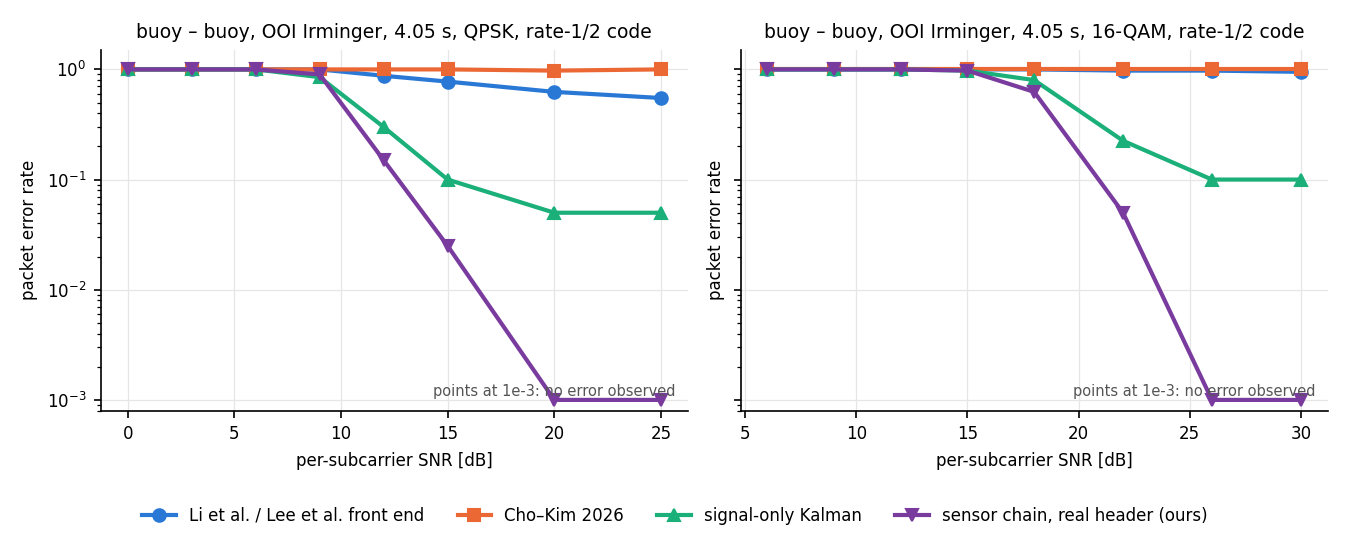
\includegraphics[width=0.88\textwidth]{../code/results/figures/fig_per_long.png}

\footnotesize With 1\,s packets, signal-only Kalman and our chain are equal (no errors from 15\,dB QPSK / 22\,dB 16-QAM); Li/Lee floors in the rough sea (4--6\% QPSK, 23--55\% 16-QAM). 40 packets per point; higher statistics running.
\end{frame}

\begin{frame}{Multipath: per-path Doppler from sensors makes cancellation work \simres}
\centering
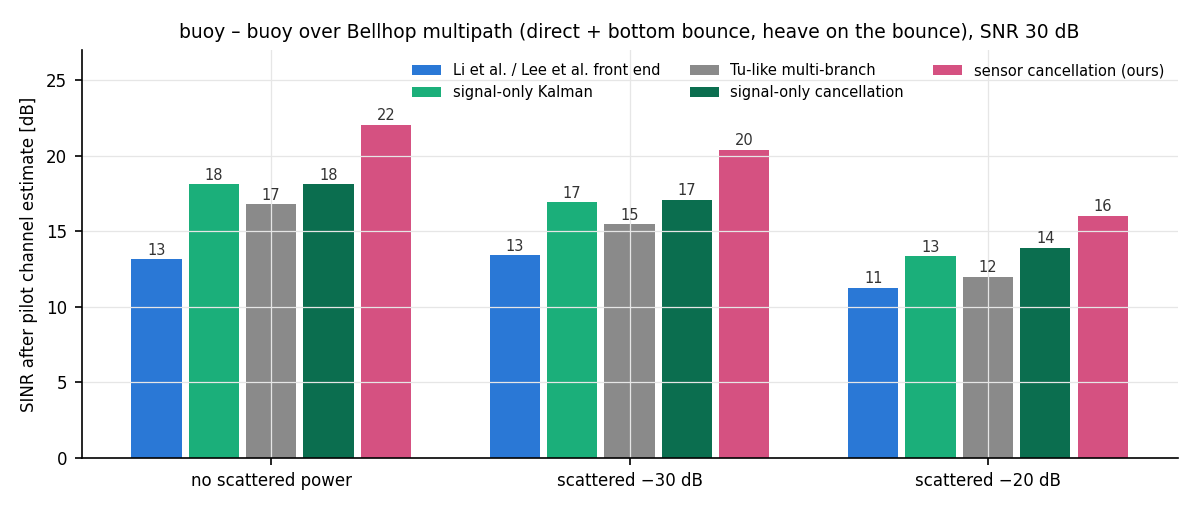
\includegraphics[width=0.85\textwidth]{../code/results/figures/fig_multipath.png}

\footnotesize The bottom bounce carries both buoys' heave $\times \sin 10^\circ$: one resampling cannot fix two paths. Sensor-predicted cancellation: +3--4\,dB over every signal-only receiver, PER 0.05--0.10 vs 0.20--0.30 at 20--30\,dB. \alert{Needs path angles within $\approx$0.5--1$^\circ$}; delays from the signal.
\end{frame}

\begin{frame}{Side information: a few tens of bits, read before the Doppler is known \simres}
\begin{columns}[T]
\begin{column}{0.58\textwidth}
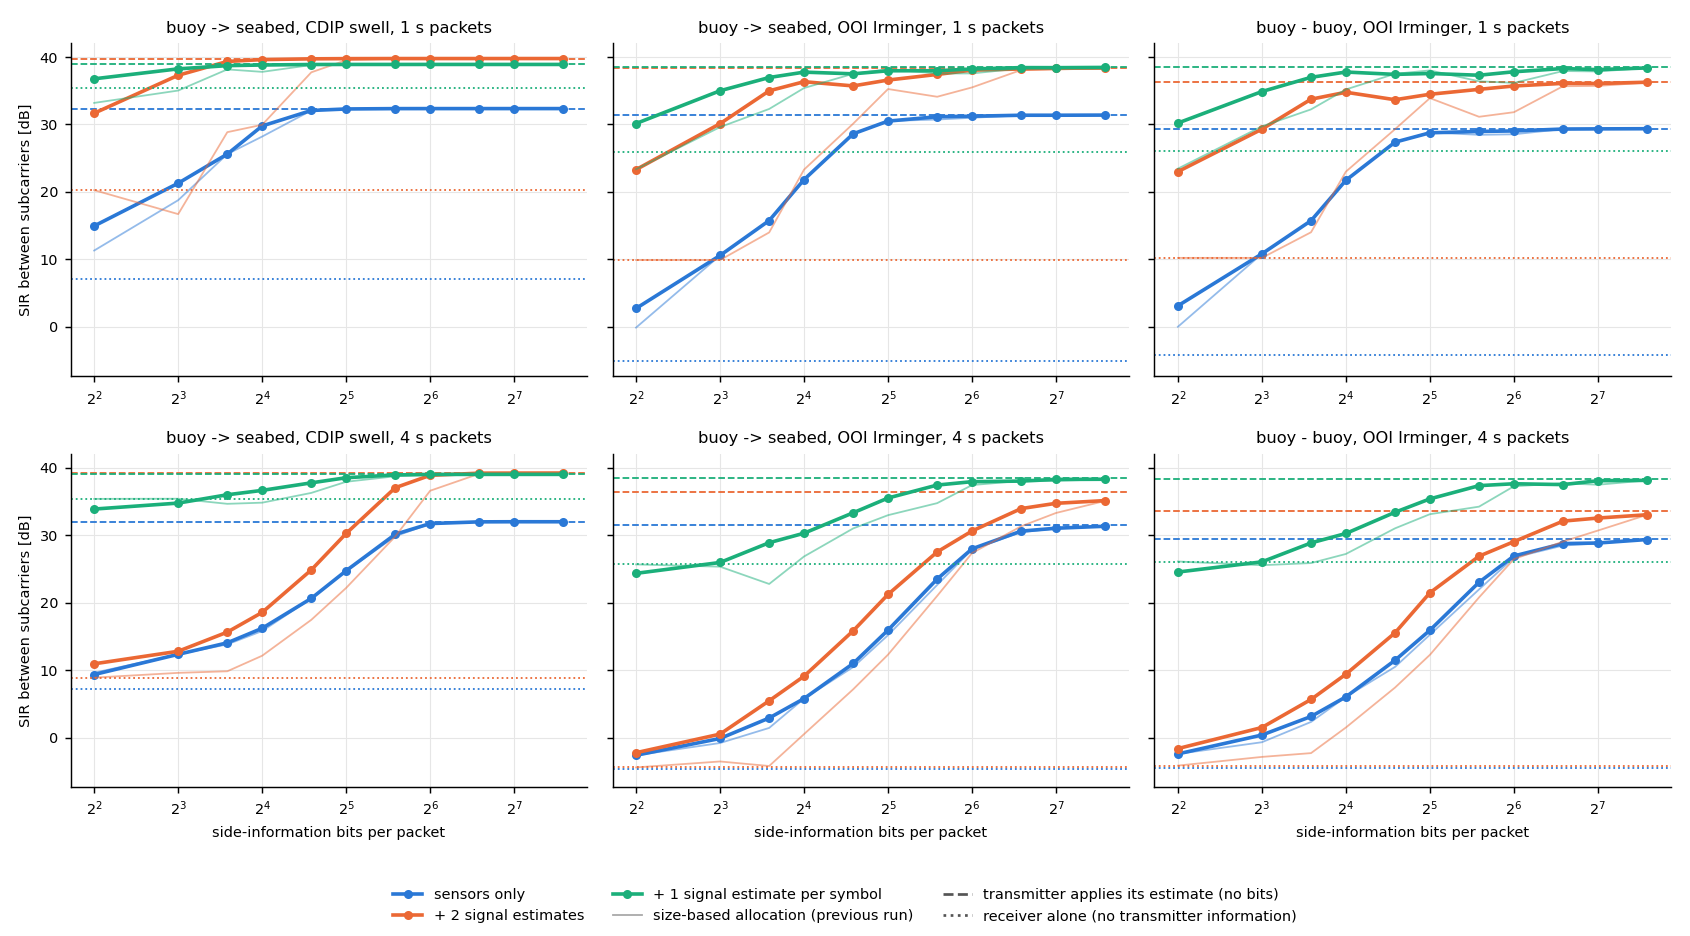
\includegraphics[width=\linewidth]{../code/results/e1_sideinfo/sir_vs_bits_stage_alloc.png}
\end{column}
\begin{column}{0.38\textwidth}
\footnotesize
\begin{itemize}\setlength{\itemsep}{2pt}
\item \alert{10--30 bits per second} of packet reach the gain of the transmitter compensating itself ($<$1\% of the packet; pilots in every symbol: 25\%)
\item what to send depends on what the receiver estimates itself (stage-aware allocation, up to 2.7$\times$ fewer bits)
\item header (DBPSK, CRC-8) read in 100\% of packets at $\geq$5\,dB, 95--100\% at 0\,dB (16--32 bits); then the chain equals ideal side information
\end{itemize}
\end{column}
\end{columns}
\end{frame}

\begin{frame}{Where we stand: claim and requirements}
\begin{columns}[T]
\begin{column}{0.52\textwidth}
\footnotesize
\textbf{Claim} \simres: sensor-aided Doppler estimation removes the error floor that the best signal-only receiver keeps when the sea is rough, both ends move and packets are long, and makes per-path cancellation possible in multipath; it matches the best signal-only receiver elsewhere (Lee et al.'s regime).

\medskip
\textbf{Not yet:} statistics for figures (running), multi-user, DESERT, writing.
\end{column}
\begin{column}{0.44\textwidth}
\footnotesize
\textbf{Requirements}
\begin{itemize}\setlength{\itemsep}{1pt}
\item IMU drift $\lesssim$0.01--0.1\,m/s; latency $\lesssim$100\,ms (bridged); lever arm from the gyro
\item side information 32 bits (1\,s) -- 96 bits (4\,s); +32 bits vertical for multipath
\item path angles within $\approx$0.5--1$^\circ$
\item scattered surface power $\lesssim -20$\,dB (else a floor for all)
\end{itemize}
\end{column}
\end{columns}
\end{frame}

\begin{frame}{Where sensor-aided estimation matters: our regime vs Lee et al.\ 2026}
\scriptsize\setlength{\tabcolsep}{4pt}\renewcommand{\arraystretch}{1.05}
\begin{tabular}{@{}L{0.26\textwidth}L{0.33\textwidth}L{0.33\textwidth}@{}}
\toprule
 & \textbf{Lee et al.\ 2026 (field)} & \textbf{Where a better estimate pays}\\
\midrule
SNR / modulation & $\approx$9\,dB, QPSK + turbo & high SNR, 16-QAM and above (residual 0.2\,$\Delta f$ $\approx$ 9\,dB SIR is binding)\\
Frame length & 0.875\,s & $>$1\,s (one model per frame cannot follow waves)\\
Sea / platform & sea state 3, small buoy, receiver only moving & rough seas, large buoys, both ends moving, AUVs\\
Overhead & preamble + pilots & short preamble, few pilots, narrow search\\
Acquisition & raw Doppler up to 0.6\,$\Delta f$, near their failure point & sensor prior centres the search\\
\bottomrule
\end{tabular}

\medskip
\footnotesize \claim\ sensor-aided estimation helps where signal estimation is weak or costly; it must not lose elsewhere (AsyMov objection). Coded PER confirms it on Lee's own metric (Results).
\end{frame}

\begin{frame}{Theory and evaluation}
\begin{columns}[T,onlytextwidth]
\begin{column}{0.5\textwidth}
\footnotesize
\textbf{Theory}
\begin{description}\setlength{\itemsep}{1pt}
\item[T1] estimation error $\to$ interference \simres\ done
\item[T2] residual vs side-information bits \simres\ simulated; closed form open
\item[T3] fused error and bound with / without sensor prior \open
\item[T4] staleness: why feedback fails \simres\ done
\end{description}
\end{column}
\begin{column}{0.46\textwidth}
\footnotesize
\textbf{Evaluation}
\begin{itemize}\setlength{\itemsep}{1pt}
\item real buoy motion (CDIP, OOI), modelled AUVs
\item OFDM simulator, Bellhop channels, scattered-surface floor
\item SIR, then coded PER; overhead (pilots, bits); search complexity
\item network level: DESERT estimation-aware PHY
\end{itemize}
\end{column}
\end{columns}
\end{frame}

\begin{frame}{Risks}
\begin{columns}[T]
\begin{column}{0.5\textwidth}
\footnotesize
\textbf{Noise-limited links} (Lee et al.\ 2026): the frame-level estimate is enough there; state the regime, show coded PER.

\medskip
\textbf{Signal can beat sensors} (AsyMov): fusion must gain where the signal is weak or costly and not lose elsewhere.

\medskip
\textbf{Chicken and egg:} solved in simulation --- header read in 95--100\% of packets from 0\,dB, fallback to signal-only otherwise.
\end{column}
\begin{column}{0.46\textwidth}
\footnotesize
\textbf{Scattered-surface floor:} above $\approx -20$\,dB, accuracy gains vanish.

\medskip
\textbf{Radio prior art} (GNSS / IMU-aided Doppler, patents): claim ``first for UWA, with real wave motion, side-information sizing and fusion''.

\medskip
\textbf{Data:} motion real, channels simulated.
\end{column}
\end{columns}
\end{frame}

% ===========================================================
\section{Questions for the group}

\begin{frame}{Questions for the group}
\small
\begin{itemize}
\item Which nodes have an IMU / INS, and can the modem read it at symbol rate with known latency?
\item How many header bits per packet can side information take?
\item Is transmit-side pre-compensation (applying the estimate) in scope next to side information (sending it)?
\item {\color{mute}Decided: SIR first, coded PER next --- now urgent to answer Lee et al.\ 2026.}
\end{itemize}
\end{frame}

\end{document}
